\documentclass[14pt]{beamer}
\usepackage[utf8]{inputenc}
\usetheme{Singapore}
\usepackage{amsmath}
\usepackage{amsfonts}
\usepackage{amssymb}
\usepackage{graphicx}
\usepackage[demo]{graphicx}
\usepackage{caption}
\usepackage{subcaption}
\hypersetup{
    colorlinks=true,
    linkcolor=blue,
    filecolor=magenta,      
    urlcolor=cyan,
}
\usepackage{tikz} %Tikz Graphs
\usepackage{capt-of} %Caption for Tikz
\usetikzlibrary{decorations.pathreplacing}
\usetikzlibrary{patterns}

%\author[María Gabriela Ertola Navajas]{Gabriela Ertola Navajas}
\title{ECONOM\'{I}A I (E010)}
\subtitle{Tema 2 \\ Escasez y elección}
%\setbeamercovered{transparent} 
%\setbeamertemplate{navigation symbols}{} 
%\institute{} 
%\date{} 
%\subject{} 
\setbeamertemplate{navigation symbols}{}

\begin{document}

\begin{frame}
\frametitle{ECONOM\'{I}A I (E010) \\ \vspace{12mm} Video complementario }
\centering \\ \vspace{4mm} 
Tema 2 \\ Teoría del consumidor \\ \vspace{4mm} Efecto ingreso y efecto sustitutución
\includegraphics[scale=0.25]{Figures/logoUDESA.jpg} 
\end{frame}

\begin{frame}
\frametitle{1. Partimos de un equilibrio}
\begin{center}
\begin{figure}[H]
\renewcommand{\figurename}{Figure}
\begin{center}
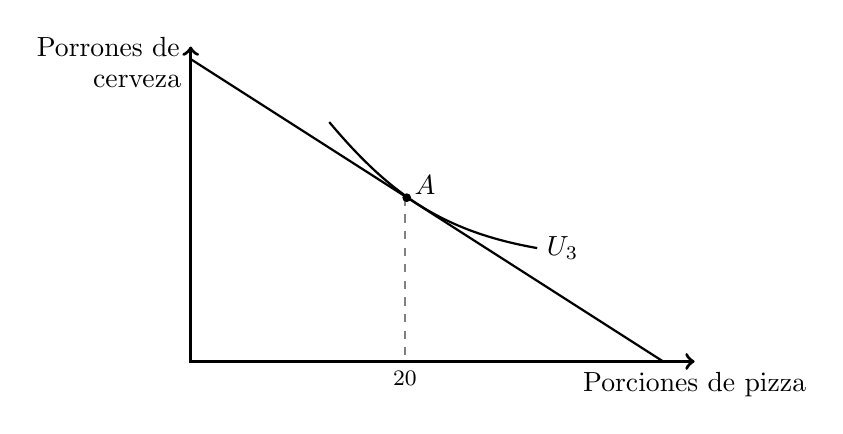
\begin{tikzpicture}[scale=0.8]
\draw[very thick,<->] (0,5) node[left]{Porrones de}--(0,0)--(8,0) node[below]{Porciones de pizza};
\node [below left] at (0,4.7) {cerveza};
\draw [thick] (2.2,3.8) to [out=310,in=170] (5.5,1.8);
\node [right] at (5.5,1.8) {$U_3$};
%\draw [thick] (0.3,4.5) to [out=290,in=165] (3.1,1.6);
%\node [right] at (3.1,1.6) {$U_2$};
\node[below] at (3.4,0) {\footnotesize 20};
%\node[below] at (0.8,0) {\footnotesize 5};
%\node[left] at (0,2.6) {\footnotesize 10};
%\node[left] at (0,3.25) {\footnotesize 15};
%\node [right] at (6,1.1) {$C$};
%\node [right] at (0.5,4.1) {$\texttt{I}$};
\draw [thick] (0,4.8) -- (7.5,0);
%\draw [thick] (0,4.8) -- (2.7,0);
%\draw[thick, dashed,gray](0.9,3.2)--(0.9,0);
\draw[thick, dashed,gray](3.4,2.6)--(3.4,0);
%\draw[thick, dashed,gray](0.9,3.25)--(0,3.25);
%\draw[thick, dashed,gray](3.43,2.6)--(0,2.6);
%\draw [thick] (0,3.3) -- (5.3,0);
%\draw[dashed](2.2,1.9)--(2.2,0);
%\node [above] at (2.4,1.9) {$C$};
%\draw[fill] (2.22,1.9) circle [radius =0.06];
%\node [above] at (3,1.7) {$\texttt{I}$};
%\node [right] at (0.8,3.5) {$B$};
%\draw[fill] (0.9,3.25) circle [radius =0.06];
\node [right] at (3.4,2.8) {$A$};
\draw[fill] (3.43,2.6) circle [radius =0.06];
\end{tikzpicture}
\end{center}
\end{figure}
\end{center}
\end{frame}

\begin{frame}
\frametitle{2. Ante un aumento en el precio...}
\begin{itemize}
    \item El consumidor va a sentirse menos rico porque su conjunto factible se ha reducido \vspace{1mm}
    \item El cambio en el precio de un bien también altera los precios relativos \vspace{1mm}
    \item Habrá una nueva canasta óptima para el consumidor  \vspace{1mm}
\end{itemize} 
\end{frame}


\begin{frame}
\frametitle{3. Aumento en el precio de la pizza}
\begin{center}
\begin{figure}[H]
\renewcommand{\figurename}{Figure}
\begin{center}
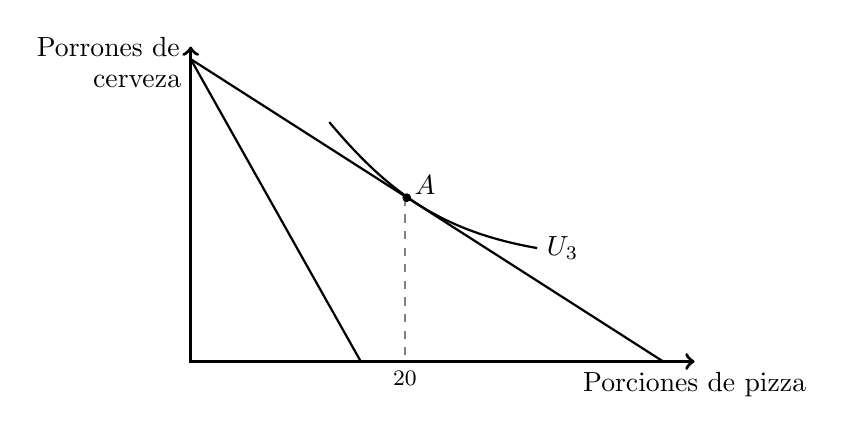
\begin{tikzpicture}[scale=0.8]
\draw[very thick,<->] (0,5) node[left]{Porrones de}--(0,0)--(8,0) node[below]{Porciones de pizza};
\node [below left] at (0,4.7) {cerveza};
\draw [thick] (2.2,3.8) to [out=310,in=170] (5.5,1.8);
\node [right] at (5.5,1.8) {$U_3$};
%\draw [thick] (0.3,4.5) to [out=290,in=165] (3.1,1.6);
%\node [right] at (3.1,1.6) {$U_2$};
\node[below] at (3.4,0) {\footnotesize 20};
%\node[below] at (0.8,0) {\footnotesize 5};
%\node[left] at (0,2.6) {\footnotesize 10};
%\node[left] at (0,3.25) {\footnotesize 15};

%\node [right] at (6,1.1) {$C$};
%\node [right] at (0.5,4.1) {$\texttt{I}$};
\draw [thick] (0,4.8) -- (7.5,0);
\draw [thick] (0,4.8) -- (2.7,0);
%\draw[thick, dashed,gray](0.9,3.2)--(0.9,0);
\draw[thick, dashed,gray](3.4,2.6)--(3.4,0);
%\draw[thick, dashed,gray](0.9,3.25)--(0,3.25);
%\draw[thick, dashed,gray](3.43,2.6)--(0,2.6);
%\draw [thick] (0,3.3) -- (5.3,0);
%\draw[dashed](2.2,1.9)--(2.2,0);
%\node [above] at (2.4,1.9) {$C$};
%\draw[fill] (2.22,1.9) circle [radius =0.06];
%\node [above] at (3,1.7) {$\texttt{I}$};
%\node [right] at (0.8,3.5) {$B$};
%\draw[fill] (0.9,3.25) circle [radius =0.06];
\node [right] at (3.4,2.8) {$A$};
\draw[fill] (3.43,2.6) circle [radius =0.06];
\end{tikzpicture}
\end{center}
\end{figure}
\end{center}
\end{frame}


\begin{frame}
\frametitle{4. Nueva canasta óptima: B}
\begin{center}
\begin{figure}[H]
\renewcommand{\figurename}{Figure}
\begin{center}
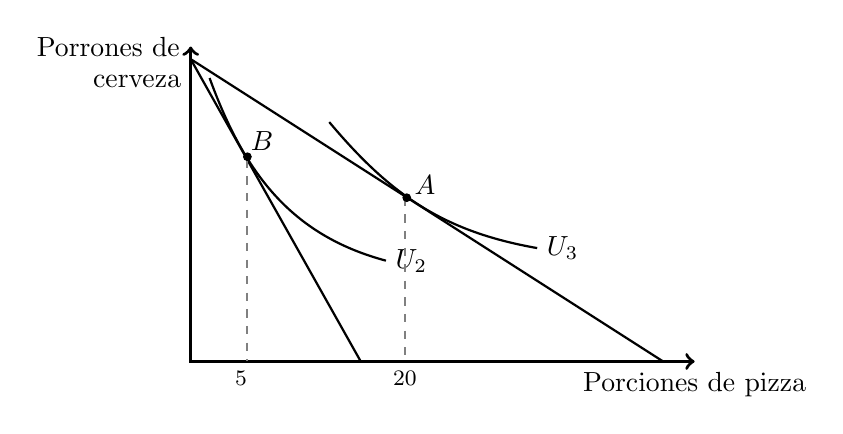
\begin{tikzpicture}[scale=0.8]
\draw[very thick,<->] (0,5) node[left]{Porrones de}--(0,0)--(8,0) node[below]{Porciones de pizza};
\node [below left] at (0,4.7) {cerveza};
\draw [thick] (2.2,3.8) to [out=310,in=170] (5.5,1.8);
\node [right] at (5.5,1.8) {$U_3$};
\draw [thick] (0.3,4.5) to [out=290,in=165] (3.1,1.6);
\node [right] at (3.1,1.6) {$U_2$};
\node[below] at (3.4,0) {\footnotesize 20};
\node[below] at (0.8,0) {\footnotesize 5};
%\node[left] at (0,2.6) {\footnotesize 10};
%\node[left] at (0,3.25) {\footnotesize 15};

%\node [right] at (6,1.1) {$C$};
%\node [right] at (0.5,4.1) {$\texttt{I}$};
\draw [thick] (0,4.8) -- (7.5,0);
\draw [thick] (0,4.8) -- (2.7,0);
\draw[thick, dashed,gray](0.9,3.2)--(0.9,0);
\draw[thick, dashed,gray](3.4,2.6)--(3.4,0);
%\draw[thick, dashed,gray](0.9,3.25)--(0,3.25);
%\draw[thick, dashed,gray](3.43,2.6)--(0,2.6);
%\draw [thick] (0,3.3) -- (5.3,0);
%\draw[dashed](2.2,1.9)--(2.2,0);
%\node [above] at (2.4,1.9) {$C$};
%\draw[fill] (2.22,1.9) circle [radius =0.06];
%\node [above] at (3,1.7) {$\texttt{I}$};
\node [right] at (0.8,3.5) {$B$};
\draw[fill] (0.9,3.25) circle [radius =0.06];
\node [right] at (3.4,2.8) {$A$};
\draw[fill] (3.43,2.6) circle [radius =0.06];
\end{tikzpicture}
\end{center}
\end{figure}
\end{center}
\end{frame}

\begin{frame}
\frametitle{5. Efecto Total}
\begin{center}
\begin{figure}[H]
\renewcommand{\figurename}{Figure}
\begin{center}
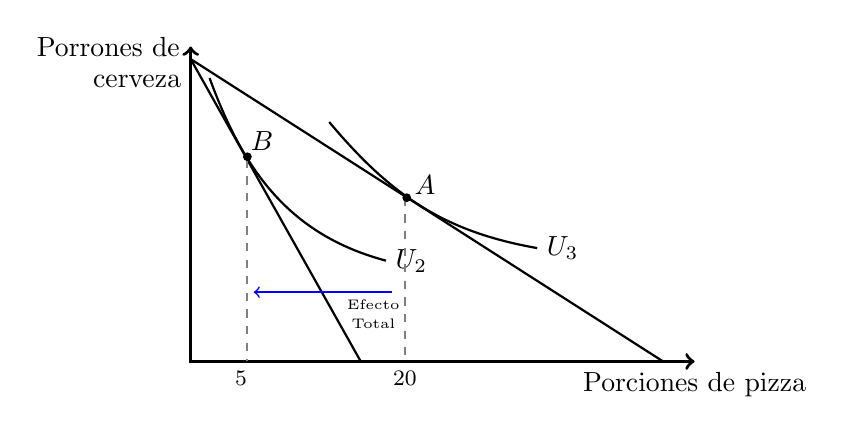
\begin{tikzpicture}[scale=0.8]
\draw[very thick,<->] (0,5) node[left]{Porrones de}--(0,0)--(8,0) node[below]{Porciones de pizza};
\node [below left] at (0,4.7) {cerveza};
\draw [thick] (2.2,3.8) to [out=310,in=170] (5.5,1.8);
\node [right] at (5.5,1.8) {$U_3$};
\draw [thick] (0.3,4.5) to [out=290,in=165] (3.1,1.6);
\node [right] at (3.1,1.6) {$U_2$};
\node[below] at (3.4,0) {\footnotesize 20};
%\node[below] at (2.22,0) {\footnotesize 10};
\node[below] at (0.8,0) {\footnotesize 5};
%\node[left] at (0,1.9) {\footnotesize 7};
%\node[left] at (0,2.6) {\footnotesize 10};
%\node[left] at (0,3.25) {\footnotesize 15};

\draw [thick] (0,4.8) -- (7.5,0);
\draw [thick] (0,4.8) -- (2.7,0);
\draw[thick, dashed,gray](0.9,3.2)--(0.9,0);
\draw[thick, dashed,gray](3.4,2.6)--(3.4,0);
%\draw[thick, dashed,gray](0.9,3.25)--(0,3.25);
%\draw[thick, dashed,gray](3.43,2.6)--(0,2.6);
%\draw[thick, dashed,gray](2.22,1.9)--(2.22,0);
%\draw[thick, dashed,gray](0,1.9)--(2.22,1.9);
%\draw [thick, gray] (0,3.3) -- (5.3,0);

\draw[semithick, blue, <-] (1,1.1)--(3.2,1.1);
\node[] at (2.9,0.9){\tiny Efecto};
\node[] at (2.9,0.6){\tiny Total};

%\draw[semithick, blue, <-] (1,1.1)--(2,1.1);
%\node[] at (1.5,0.9){\tiny Efecto};
%\node[] at (1.5,0.6){\tiny Sustitución};

%\node [above] at (2.4,1.9) {$C$};
%\draw[fill] (2.22,1.9) circle [radius =0.06];
%\node [above] at (3,1.7) {$\texttt{I}$};
\node [right] at (0.8,3.5) {$B$};
\draw[fill] (0.9,3.25) circle [radius =0.06];
\node [right] at (3.4,2.8) {$A$};
\draw[fill] (3.43,2.6) circle [radius =0.06];
\end{tikzpicture}
\end{center}

\end{figure}
\end{center}
\end{frame}

\begin{frame}
\frametitle{6. Efecto ingreso y efecto sustitución}
\begin{itemize}
    \item Un aumento en el precio de la pizza
    \begin{itemize}
        \item Disminuye el poder de compra, disminuyendo el nivel de utilidad
        \item Aumenta el costo de oportunidad de comprar cerveza
    \end{itemize}
    \item Tenemos dos efectos
    \begin{itemize}
    \item Efecto ingreso \\
    - La restricción presupuestaria se desplaza hacia adentro \\
    - El efecto que el ingreso menor tendría si no hubiera cambios en el costo de oportunidad
    \item Efecto sustitución \\
    - La pendiente de la restricción presupuestaria (TMT) aumenta: el efecto del cambio en el costo de oportunidad, dado el nuevo nivel de utilidad
    \end{itemize}
\end{itemize} 
\end{frame}

\begin{frame}
\frametitle{7. Y si le damos menos dinero para que esté sobre $U_2$, ¿elige B?}
\begin{center}
\begin{figure}[H]
\renewcommand{\figurename}{Figure}
\begin{center}
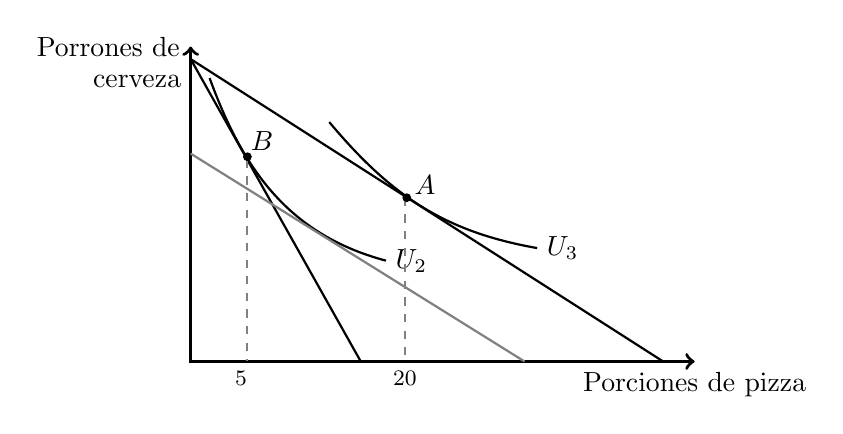
\begin{tikzpicture}[scale=0.8]
\draw[very thick,<->] (0,5) node[left]{Porrones de}--(0,0)--(8,0) node[below]{Porciones de pizza};
\node [below left] at (0,4.7) {cerveza};
\draw [thick] (2.2,3.8) to [out=310,in=170] (5.5,1.8);
\node [right] at (5.5,1.8) {$U_3$};
\draw [thick] (0.3,4.5) to [out=290,in=165] (3.1,1.6);
\node [right] at (3.1,1.6) {$U_2$};
\node[below] at (3.4,0) {\footnotesize 20};
%\node[below] at (2.22,0) {\footnotesize 10};
\node[below] at (0.8,0) {\footnotesize 5};
%\node[left] at (0,1.9) {\footnotesize 7};
%\node[left] at (0,2.6) {\footnotesize 10};
%\node[left] at (0,3.25) {\footnotesize 15};

\draw [thick] (0,4.8) -- (7.5,0);
\draw [thick] (0,4.8) -- (2.7,0);
\draw[thick, dashed,gray](0.9,3.2)--(0.9,0);
\draw[thick, dashed,gray](3.4,2.6)--(3.4,0);
%\draw[thick, dashed,gray](0.9,3.25)--(0,3.25);
%\draw[thick, dashed,gray](3.43,2.6)--(0,2.6);
%\draw[thick, dashed,gray](2.22,1.9)--(2.22,0);
%\draw[thick, dashed,gray](0,1.9)--(2.22,1.9);
\draw [thick, gray] (0,3.3) -- (5.3,0);

%\draw[semithick, blue, <-] (1,1.1)--(3.2,1.1);
%\node[] at (2.9,0.9){\tiny Efecto};
%\node[] at (2.9,0.6){\tiny Total};

%\draw[semithick, blue, <-] (1,1.1)--(2,1.1);
%\node[] at (1.5,0.9){\tiny Efecto};
%\node[] at (1.5,0.6){\tiny Sustitución};

%\node [above] at (2.4,1.9) {$C$};
%\draw[fill] (2.22,1.9) circle [radius =0.06];
%\node [above] at (3,1.7) {$\texttt{I}$};
\node [right] at (0.8,3.5) {$B$};
\draw[fill] (0.9,3.25) circle [radius =0.06];
\node [right] at (3.4,2.8) {$A$};
\draw[fill] (3.43,2.6) circle [radius =0.06];
\end{tikzpicture}
\end{center}

\end{figure}
\end{center}
\end{frame}


\begin{frame}
\frametitle{8. No, elige C}
\begin{center}
\begin{figure}[H]
\renewcommand{\figurename}{Figure}
\begin{center}
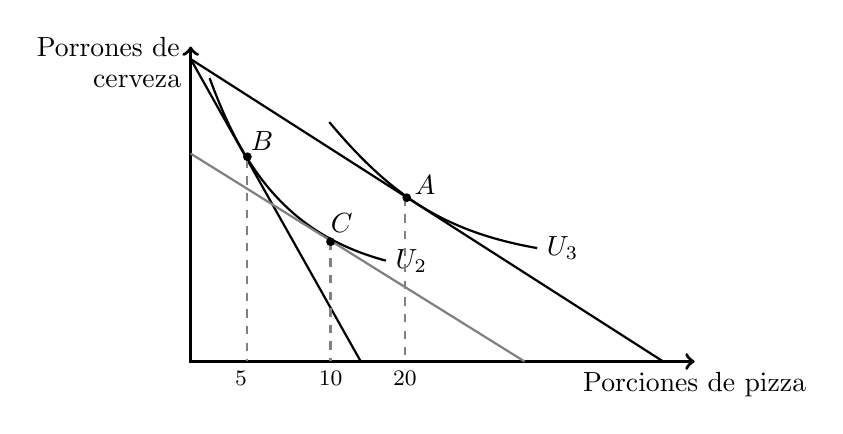
\begin{tikzpicture}[scale=0.8]
\draw[very thick,<->] (0,5) node[left]{Porrones de}--(0,0)--(8,0) node[below]{Porciones de pizza};
\node [below left] at (0,4.7) {cerveza};
\draw [thick] (2.2,3.8) to [out=310,in=170] (5.5,1.8);
\node [right] at (5.5,1.8) {$U_3$};
\draw [thick] (0.3,4.5) to [out=290,in=165] (3.1,1.6);
\node [right] at (3.1,1.6) {$U_2$};
\node[below] at (3.4,0) {\footnotesize 20};
\node[below] at (2.22,0) {\footnotesize 10};
\node[below] at (0.8,0) {\footnotesize 5};
%\node[left] at (0,1.9) {\footnotesize 7};
%\node[left] at (0,2.6) {\footnotesize 10};
%\node[left] at (0,3.25) {\footnotesize 15};

\draw [thick] (0,4.8) -- (7.5,0);
\draw [thick] (0,4.8) -- (2.7,0);
\draw[thick, dashed,gray](0.9,3.2)--(0.9,0);
\draw[thick, dashed,gray](3.4,2.6)--(3.4,0);
%\draw[thick, dashed,gray](0.9,3.25)--(0,3.25);
%\draw[thick, dashed,gray](3.43,2.6)--(0,2.6);
\draw[thick, dashed,gray](2.22,1.9)--(2.22,0);
%\draw[thick, dashed,gray](0,1.9)--(2.22,1.9);
\draw [thick, gray] (0,3.3) -- (5.3,0);

%\draw[semithick, blue, <-] (1,1.1)--(3.2,1.1);
%\node[] at (2.9,0.9){\tiny Efecto};
%\node[] at (2.9,0.6){\tiny Total};

%\draw[semithick, blue, <-] (1,1.1)--(2,1.1);
%\node[] at (1.5,0.9){\tiny Efecto};
%\node[] at (1.5,0.6){\tiny Sustitución};

\node [above] at (2.4,1.9) {$C$};
\draw[fill] (2.22,1.9) circle [radius =0.06];
%\node [above] at (3,1.7) {$\texttt{I}$};
\node [right] at (0.8,3.5) {$B$};
\draw[fill] (0.9,3.25) circle [radius =0.06];
\node [right] at (3.4,2.8) {$A$};
\draw[fill] (3.43,2.6) circle [radius =0.06];
\end{tikzpicture}
\end{center}

\end{figure}
\end{center}
\end{frame}

\begin{frame}
\frametitle{9. El efecto ingreso}
\begin{center}
\begin{figure}[H]
\renewcommand{\figurename}{Figure}
\begin{center}
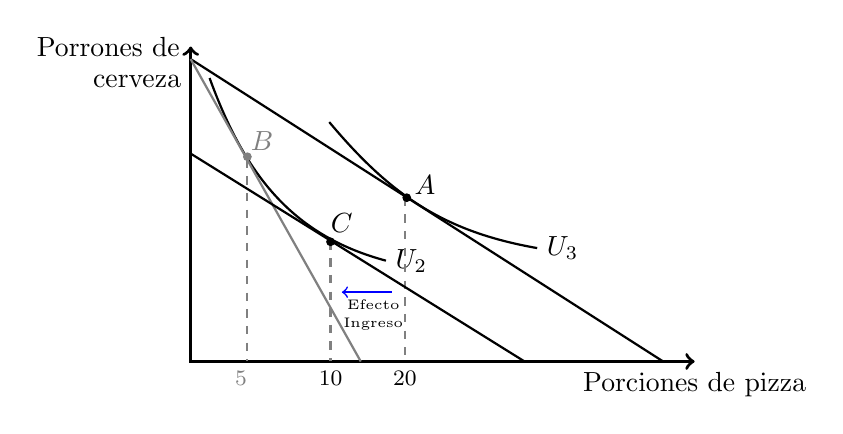
\begin{tikzpicture}[scale=0.8]
\draw[very thick,<->] (0,5) node[left]{Porrones de}--(0,0)--(8,0) node[below]{Porciones de pizza};
\node [below left] at (0,4.7) {cerveza};
\draw [thick] (2.2,3.8) to [out=310,in=170] (5.5,1.8);
\node [right] at (5.5,1.8) {$U_3$};
\draw [thick] (0.3,4.5) to [out=290,in=165] (3.1,1.6);
\node [right] at (3.1,1.6) {$U_2$};
\node[below] at (3.4,0) {\footnotesize 20};
\node[below] at (2.22,0) {\footnotesize 10};
\node[below,gray] at (0.8,0) {\footnotesize 5};
%\node[left] at (0,1.9) {\footnotesize 7};
%\node[left] at (0,2.6) {\footnotesize 10};
%\node[left] at (0,3.25) {\footnotesize 15};

\draw [thick] (0,4.8) -- (7.5,0);
\draw [thick,gray] (0,4.8) -- (2.7,0);
\draw[thick, dashed,gray](0.9,3.2)--(0.9,0);
\draw[thick, dashed,gray](3.4,2.6)--(3.4,0);
%\draw[thick, dashed,gray](0.9,3.25)--(0,3.25);
%\draw[thick, dashed,gray](3.43,2.6)--(0,2.6);
\draw[thick, dashed,gray](2.22,1.9)--(2.22,0);
%\draw[thick, dashed,gray](0,1.9)--(2.22,1.9);
\draw [thick] (0,3.3) -- (5.3,0);

%\draw[semithick, blue, <-] (1,1.1)--(3.2,1.1);
%\node[] at (2.9,0.9){\tiny Efecto};
%\node[] at (2.9,0.6){\tiny Total};

\draw[semithick, blue, <-] (2.4,1.1)--(3.2,1.1);
\node[] at (2.9,0.9){\tiny Efecto};
\node[] at (2.9,0.6){\tiny Ingreso};

%\draw[semithick, blue, <-] (1,1.1)--(2,1.1);
%\node[] at (1.5,0.9){\tiny Efecto};
%\node[] at (1.5,0.6){\tiny Sustitución};

\node [above] at (2.4,1.9) {$C$};
\draw[fill] (2.22,1.9) circle [radius =0.06];
%\node [above] at (3,1.7) {$\texttt{I}$};
\node [right,gray] at (0.8,3.5) {$B$};
\draw[fill,gray] (0.9,3.25) circle [radius =0.06];
\node [right] at (3.4,2.8) {$A$};
\draw[fill] (3.43,2.6) circle [radius =0.06];
\end{tikzpicture}
\end{center}

\end{figure}
\end{center}
\end{frame}


\begin{frame}
\frametitle{10. El efecto sustitución}
\begin{center}
\begin{figure}[H]
\renewcommand{\figurename}{Figure}
\begin{center}
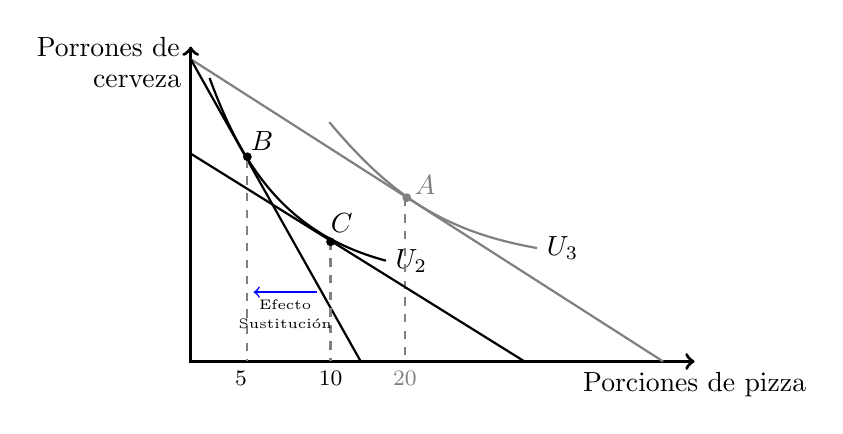
\begin{tikzpicture}[scale=0.8]
\draw[very thick,<->] (0,5) node[left]{Porrones de}--(0,0)--(8,0) node[below]{Porciones de pizza};
\node [below left] at (0,4.7) {cerveza};
\draw [thick,gray] (2.2,3.8) to [out=310,in=170] (5.5,1.8);
\node [right] at (5.5,1.8) {$U_3$};
\draw [thick] (0.3,4.5) to [out=290,in=165] (3.1,1.6);
\node [right] at (3.1,1.6) {$U_2$};
\node[below,gray] at (3.4,0) {\footnotesize 20};
\node[below] at (2.22,0) {\footnotesize 10};
\node[below] at (0.8,0) {\footnotesize 5};
%\node[left] at (0,1.9) {\footnotesize 7};
%\node[left] at (0,2.6) {\footnotesize 10};
%\node[left] at (0,3.25) {\footnotesize 15};

\draw [thick,gray] (0,4.8) -- (7.5,0);
\draw [thick] (0,4.8) -- (2.7,0);
\draw[thick, dashed,gray](0.9,3.2)--(0.9,0);
\draw[thick, dashed,gray](3.4,2.6)--(3.4,0);
%\draw[thick, dashed,gray](0.9,3.25)--(0,3.25);
%\draw[thick, dashed,gray](3.43,2.6)--(0,2.6);
\draw[thick, dashed,gray](2.22,1.9)--(2.22,0);
%\draw[thick, dashed,gray](0,1.9)--(2.22,1.9);
\draw [thick] (0,3.3) -- (5.3,0);

%\draw[semithick, blue, <-] (1,1.1)--(3.2,1.1);
%\node[] at (2.9,0.9){\tiny Efecto};
%\node[] at (2.9,0.6){\tiny Total};

%\draw[semithick, blue, <-] (2.4,1.1)--(3.2,1.1);
%\node[] at (2.9,0.9){\tiny Efecto};
%\node[] at (2.9,0.6){\tiny Ingreso};

\draw[semithick, blue, <-] (1,1.1)--(2,1.1);
\node[] at (1.5,0.9){\tiny Efecto};
\node[] at (1.5,0.6){\tiny Sustitución};

\node [above] at (2.4,1.9) {$C$};
\draw[fill] (2.22,1.9) circle [radius =0.06];
%\node [above] at (3,1.7) {$\texttt{I}$};
\node [right] at (0.8,3.5) {$B$};
\draw[fill] (0.9,3.25) circle [radius =0.06];
\node [right,gray] at (3.4,2.8) {$A$};
\draw[fill,gray] (3.43,2.6) circle [radius =0.06];
\end{tikzpicture}
\end{center}
\end{figure}
\end{center}
\end{frame}


\begin{frame}
\frametitle{11. El efecto total}

\begin{center}
\begin{figure}[H]
\renewcommand{\figurename}{Figure}
\begin{center}
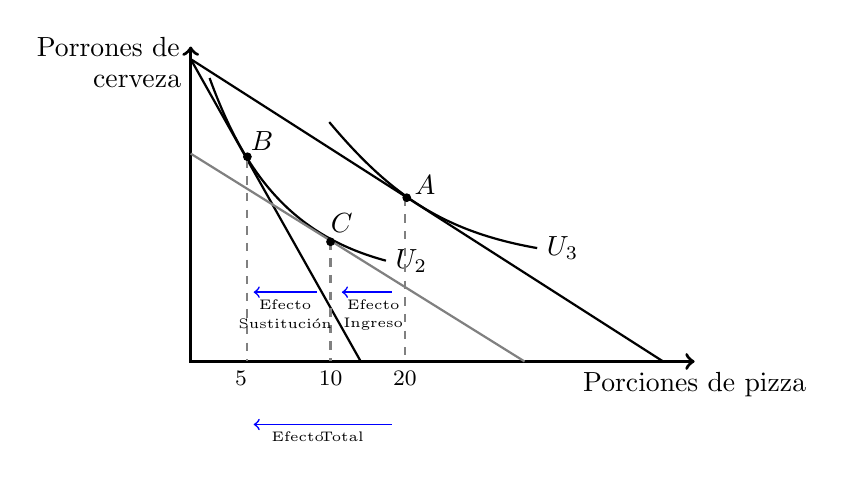
\begin{tikzpicture}[scale=0.8]
\draw[very thick,<->] (0,5) node[left]{Porrones de}--(0,0)--(8,0) node[below]{Porciones de pizza};
\node [below left] at (0,4.7) {cerveza};
\draw [thick] (2.2,3.8) to [out=310,in=170] (5.5,1.8);
\node [right] at (5.5,1.8) {$U_3$};
\draw [thick] (0.3,4.5) to [out=290,in=165] (3.1,1.6);
\node [right] at (3.1,1.6) {$U_2$};
\node[below] at (3.4,0) {\footnotesize 20};
\node[below] at (2.22,0) {\footnotesize 10};
\node[below] at (0.8,0) {\footnotesize 5};
%\node[left] at (0,1.9) {\footnotesize 7};
%\node[left] at (0,2.6) {\footnotesize 10};
%\node[left] at (0,3.25) {\footnotesize 15};

\draw [thick] (0,4.8) -- (7.5,0);
\draw [thick] (0,4.8) -- (2.7,0);
\draw[thick, dashed,gray](0.9,3.2)--(0.9,0);
\draw[thick, dashed,gray](3.4,2.6)--(3.4,0);
%\draw[thick, dashed,gray](0.9,3.25)--(0,3.25);
%\draw[thick, dashed,gray](3.43,2.6)--(0,2.6);
\draw[thick, dashed,gray](2.22,1.9)--(2.22,0);
%\draw[thick, dashed,gray](0,1.9)--(2.22,1.9);
\draw [thick, gray] (0,3.3) -- (5.3,0);

\draw[semithick, blue, <-] (1,-1)--(3.2,-1);
\node[] at (1.7,-1.2){\tiny Efecto};
\node[] at (2.4,-1.2){\tiny Total};

\draw[semithick, blue, <-] (2.4,1.1)--(3.2,1.1);
\node[] at (2.9,0.9){\tiny Efecto};
\node[] at (2.9,0.6){\tiny Ingreso};

\draw[semithick, blue, <-] (1,1.1)--(2,1.1);
\node[] at (1.5,0.9){\tiny Efecto};
\node[] at (1.5,0.6){\tiny Sustitución};

\node [above] at (2.4,1.9) {$C$};
\draw[fill] (2.22,1.9) circle [radius =0.06];
%\node [above] at (3,1.7) {$\texttt{I}$};
\node [right] at (0.8,3.5) {$B$};
\draw[fill] (0.9,3.25) circle [radius =0.06];
\node [right] at (3.4,2.8) {$A$};
\draw[fill] (3.43,2.6) circle [radius =0.06];
\end{tikzpicture}
\end{center}
\end{figure}
\end{center}
\end{frame}






\end{document}
